\section{\ac{AODCS}}
The \ac{AODCS} is used for determining and controlling the attitude and orbit of the satellites. In this section first the \ac{ADCS} design option tree is pruned in section \ref{pruneADCS}. The subsystem can be split up into four smaller parts; attitude determination (discussed in section \ref{ss:ads}), attitude control (section \ref{ss:acs}), orbit determination (section \ref{ss:ods}) and orbit control (section \ref{ss:ocs}). 

\subsection{Pruning the \acs{ADCS} design option tree}
\label{pruneADCS}
The gravity-gradient stabilisation and passive magnetic options are eliminated because they provide insufficient accuracy and do not allow pointing to a any target other than the mass or magnetic centre of the Earth. The spin stabilisation option is pruned because the satellite needs to be able to make measurements continuously. Double gimbal \acp{CMG} are also not a viable option, because they are too complex and heavy compared to the other systems.
For the attitude determination the initial measurements and magnetometers options are eliminated because of their low accuracy over time.
The pruned design option tree can be found in figure \ref{fig:pruneADCS} on page \pageref{fig:pruneADCS}.

\begin{figure}
\centering
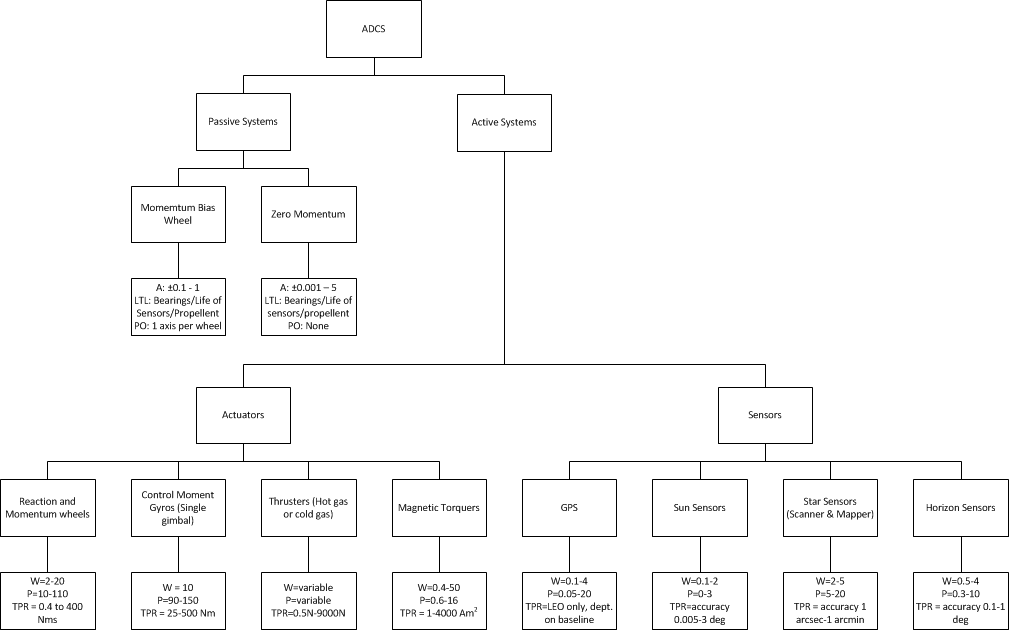
\includegraphics[width=1.0\textwidth, angle=90, bb =0 0 1009px 630px]{img/prunedADCStree.png}
\label{fig:pruneADCS}
\caption{Pruned design option tree for the \ac{ADCS}}
\end{figure}

%%%%%%%%%%%%%%%%%%%%%%%%%%%%%%%%%%%%%%%%%%%%%%%%%%%%%%%%%%%%%%%%%%%%%%%%%%%%%%%%%%%%
\subsection{\ac{ADS}}
\label{ss:ads}
The \ac{ADS} consists for a collection of sensors to determine the roll, pitch and yaw angles and rates of the satellites. The design options left after the pruning in section \ref{pruneADCS} are \ac{GPS}, Sun sensors, Star trackers and Horizon sensors. 

\ac{GPS} uses one receiver and multiple antennas, by measuring the relative positions of the different antennas the attitude of the satellite can be calculated. Most modern \ac{LEO} satellites are already carry a \ac{GPS} receiver, but a long baseline between antennas is needed for a high accuracy. 
Sun sensors use the angle towards the Sun for making their attitude measurements. The technology behind Sun sensors has been around for a long time and several micro Sun sensors are available on the market, the \ac{FOV} of a typical Sun sensor is about 120${}^{\circ}$. 
Star trackers look at a portion of the sky and uses familiar stars to determine the attitude of the satellites the system can work autonomously, but the optics required are usually quite bulky. 
Horizon sensors use the limb of the Earth, i.e. the transition of the solid Earth to cold space, to determine the attitude of the satellite. The system only works on the roll and pitch axis.

Another option is to use a complete \ac{COTS} \ac{ADCS} system like the one from Maryland Aerospace Inc. \cite{maryland}. Their IMI-100 ADACS contains everything needed for complete \ac{ADCS} with an accuracy of 1${}^\circ$. For attitude determination it uses 3 magnetometers, by adding additional sensors e.g. a ring laser gyro and a miniaturised star sensor the accuracy can reach 1-3 arcsec \cite{imi100}.

\subsubsection{Trade method}
\subsubsection{Trade criteria}
The concepts for \ac{ADS} are traded in terms of attitude determination accuracy, purchasing price, power required, size and the amount of additional development required for implementing the concept. 
\subsubsection{Weight factors}
The accuracy of the \ac{ADS} is the main driver for the choice of the system so it is given a weight factor of 9. Because the volume and power for satellites are limited they are also important with a given weight factor of 7. Although the total cost of the system is relevant, if a better performance can be achieved at a higher cost can be acceptable, weight factor 3. If a lot of work still is required to implement the system in the satellite the mission can be delayed, development gets a weight factor of 5.
\subsubsection{Trade-off}

\begin{table} [h]
\centering
\begin{tabular}{p{3cm} | c | c c c}
\textbf{Criteria} & \textbf{Weight Factor} & \textbf{Concept 1} & \textbf{Concept 2} & \textbf{Concept 3} \\ \hline \hline
Accuracy    & 9 & & & \\
Size        & 7 & & & \\
Power       & 7 & & & \\
Price       & 3 & & & \\
Development & 5 & & & \\ \hline
Weighted total    &    &  &  & 
\end{tabular} 
\caption[Trade-off attitude determination]{Trade-off graph for the attitude determination system. The weight factor signifies the importance of the criterion. Grades are given on a scale of 1 to 10, 1 being the worst, 10 the best}
\label{tab:adstradeoff}
\end{table}
%choose three concepts, trade off

%%%%%%%%%%%%%%%%%%%%%%%%%%%%%%%%%%%%%%%%%%%%%%%%%%%%%%%%%%%%%%%%%%%%%%%%%%%%%%%%%%%%
\subsection{\ac{ACS}}
\label{ss:acs}
The satellites in the constellation all need to point accurately to the Earth, a passive \ac{ACS} will therefore not be sufficient for the control of the attitude of the satellites. For active attitude control actuators are needed. After the pruning again four options remain for the attitude control. Reaction and momentum wheels, \acp{CMG}, Thusters and Magnetic torquers.

Reaction wheels are basically torque rotors with a high-inertia wheel attached to it, they can provide single axis control to a spacecraft. Momentum wheels are reaction wheels with a nominal spin rate, adding gyroscopic stiffness to two axis of the spacecraft. Chancing the spin rate gives control over the third axis.
\acp{CMG} consist of a wheel with a constant rotation speed and one or two gimbals to rotate them, pointing the direction of the momentum. This way very accurate attitude manoeuvres can be made, but complex control algorithms are needed. Usually the weight and cost of \acp{CMG} are quite high.
Thusters expel mass to induce velocity or a momentum to the satellite. The velocity can be used for keeping the orbit and will be discussed in section \ref{ss:ocs}. To be able to induce a momentum to a satellite multiple thrusters with an offset to the center of mass of the satellite. Thrusters are split up into hot gas types, which require a chemical reaction of the propellent, and cold gas types that rely on latent heat and phase change in the propellent. The power which can be generated by thrusters is high, but the fuel required will limit the lifetime of the satellite.
Magnetic torquers are magnetic coils or electromagnets generating dipole moments on the satellite. They can be used for both manoevering and desaturation of e.g. reaction wheels. Because they rely on the magnetic field of the Earth they are less useful in higher orbits.

The IMI-100 ADACS contains three miniature reaction wheels and three magnetic coils for desaturating the wheels. For a 2 kg, 2U cubesat it can provide a slew rate of $8.4^\circ/s$ \cite{imi100}.

\subsubsection{Trade method}
\subsubsection{Trade criteria}
The concepts for \ac{ACS} are traded in terms of the rate the concepts are able to adjust the attitude, attitude control accuracy, purchasing price, power required, size and the amount of additional development required for implementing the concept. 
\subsubsection{Weight factors}
A high rate in which the satellite can be controlled is convenient, but not driving, weight factor 5. Since attitude control will be used for the pointing of the instrument the accuracy is very important for the choice so it is given a weight factor of 8. Because the volume and power for satellites are limited they are also important with a given weight factor of 7. Although the total cost of the system is relevant, if a better performance can be achieved at a higher cost can be acceptable, weight factor 3. If a lot of work still is required to implement the system in the satellite the mission can be delayed, development gets a weight factor of 5.
\subsubsection{Trade-off}

\begin{table} [h]
\centering
\begin{tabular}{p{3cm} | c | c c c}
\textbf{Criteria} & \textbf{Weight Factor} & \textbf{Concept 1} & \textbf{Concept 2} & \textbf{Concept 3} \\ \hline \hline
Rate 	    & 5 & & & \\
Accuracy    & 8 & & & \\
Size        & 7 & & & \\
Power       & 7 & & & \\
Price       & 3 & & & \\
Development & 5 & & & \\ \hline
Weighted total    &    &  &  & 
\end{tabular} 
\caption[Trade-off attitude control]{Trade-off graph for the attitude control system. The weight factor signifies the importance of the criterion. Grades are given on a scale of 1 to 10, 1 being the worst, 10 the best}
\label{tab:acstradeoff}
\end{table}
%choose three concepts, trade off

%%%%%%%%%%%%%%%%%%%%%%%%%%%%%%%%%%%%%%%%%%%%%%%%%%%%%%%%%%%%%%%%%%%%%%%%%%%%%%%%%%%%
\subsection{\ac{ODS}}
\label{ss:ods}
The determination of the orbit will be discussed in section \ref{TOcommTA}.

%%%%%%%%%%%%%%%%%%%%%%%%%%%%%%%%%%%%%%%%%%%%%%%%%%%%%%%%%%%%%%%%%%%%%%%%%%%%%%%%%%%%
\subsection{\ac{OCS}}
\label{ss:ocs}
The orbit considered for the satellites is very low (for satellite orbits), therefore the drag of the atmosphere has to be taken into account. The equation for acceleration due to drag on the satellite is

\begin{equation}
a_D=-\frac{1}{2}\rho \left(C_DA/m\right)V^2
\label{eqn:atmosdrag}
\end{equation}
where $\rho$ is the density of the atmosphere, $C_D$ is the drag coefficient for the satellite (typically between 2-4), $m$ is the mass of the satellite and $V$ is the satellite's velocity with respect to the atmosphere. The orbital velocity of a circular orbit is

\begin{equation}
V_c=\sqrt{\frac{\mu}{a}}
\label{eqn:orbitalvel}
\end{equation}

where $\mu$ is the standard gravitational parameter of the Earth, $398,600.4 \,km^3/s^2$. For circular orbits the equation for $\Delta V$ per revolution can be simplified to

\begin{equation}
\Delta V_{rev}=\pi \left(C_DA/m\right)\rho a V
\label{eqn:deltaVrev}
\end{equation}

where $a$ is the orbit semi-major axis \cite{larson}.\\

Station keeping for an orbit between 400 and 500 kilometers requires a maximum $\Delta V$ of 100 m/s or on average 25 m/s \cite{deltavtu}.\\

The $\Delta V$ a propulsion system can produce is quantified by Tsiolkovsky's rocket equation

\begin{equation}
\Delta V = g I_{sp} \ln{\left(\frac{m_0}{m_0-m_p}\right)}\equiv g I_{sp} \ln{\left(\frac{m_0}{m_f}\right)} \equiv g I_{sp} \ln{\left(R\right)}
\label{eqn:tsiolkovsky}
\end{equation}

where $g$ is the Earth's gravity constant, $I_{sp}$ is the specific impulse of the engine, $m_0$ is the starting mass, $m_p$ is the mass of the fuel used, $m_f = m_0-m_p$ and the mass ratio $R$ is  ${m_0}/\left({m_0-m_p}\right)$. From this the ratio of fuel to the total mass can be derived to be

\begin{equation}
\frac{m_p}{m_0} = 1-e^{-\left(\Delta V/I_{sp}g\right)}
\label{eqn:fuelratio}
\end{equation} 